\section{Datasets}
\label{sec:datasets}
For testing the bootstrapping technique and curriculum learning as well as measuring the performance of the aerial patch framework, two datasets have been used. Both datasets involve the task of learning structured output predictions from images, specifically the task of extracting roads from aerial images. The first dataset, Massachusetts Roads Dataset, is provided by \cite{MnihThesis} and have been used in other works. The second dataset, Norwegian Roads Dataset, have been created from publicly available source specifically for this thesis. Differences, similarities and challenges of employing these datasets will be further discussed below.\\

\subsection{Massachusetts Roads Dataset}
The Massachusetts Roads Dataset contains aerial images depicting urban, suburban and rural areas in the state of Massachusetts, USA. In all the dataset consists of 1171 aerial images, where each image is $1500\times 1500$ pixels in size. The main bulk, or 1108 of these images have been randomly assigned to the training set. The remaining 49 and 14 images can be found in the test and validation set. The dataset covers an area of 2600 square kilometers in total, which gives a \ac{GSD} of 1.0 meter per pixel.\\

Each aerial image have an accompanying identically sized binary label image which indicate whether a pixel in the aerial image contains a road or not \todo{rewrite this sentence}. Road centerline vectors retrieved from the OpenStreetMap project were used to generate the labels images. The vectors were rasterized as white lines with a line thickness of 7 pixels \citep{MnihThesis}, which based on the \ac{GSD} is equivalent to 7 meters on the ground . An example from this dataset can be seen in Figure \ref{fig:mass_roads_example}.\\

\begin{figure}
\begin{subfigure}{0.48\textwidth}
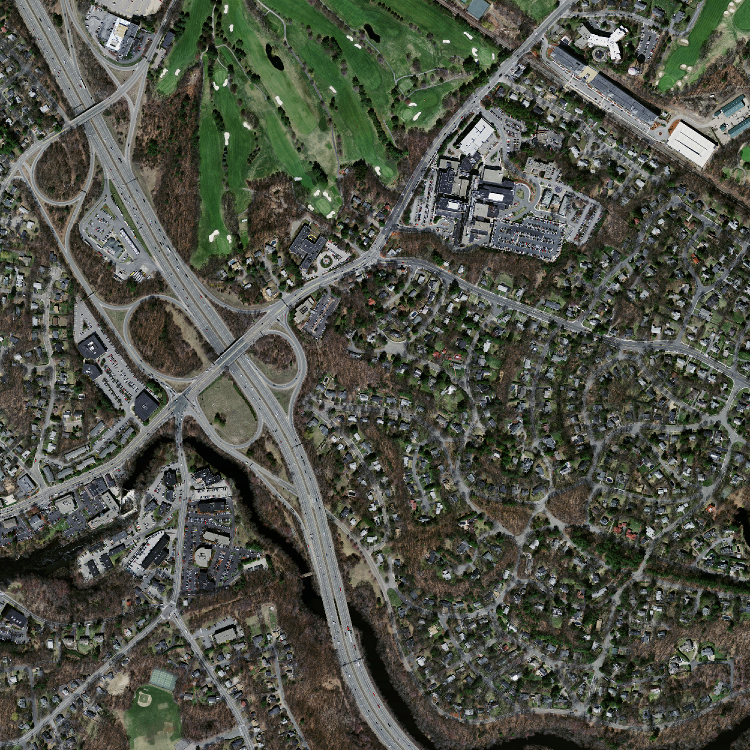
\includegraphics[width=\linewidth]{figs/datasets/Mass_roads_data_example2.png}
\caption{Aerial image} \label{fig:mass_roads_example_data}
\end{subfigure}
\hspace*{\fill} % separation between the subfigures
\begin{subfigure}{0.48\textwidth}
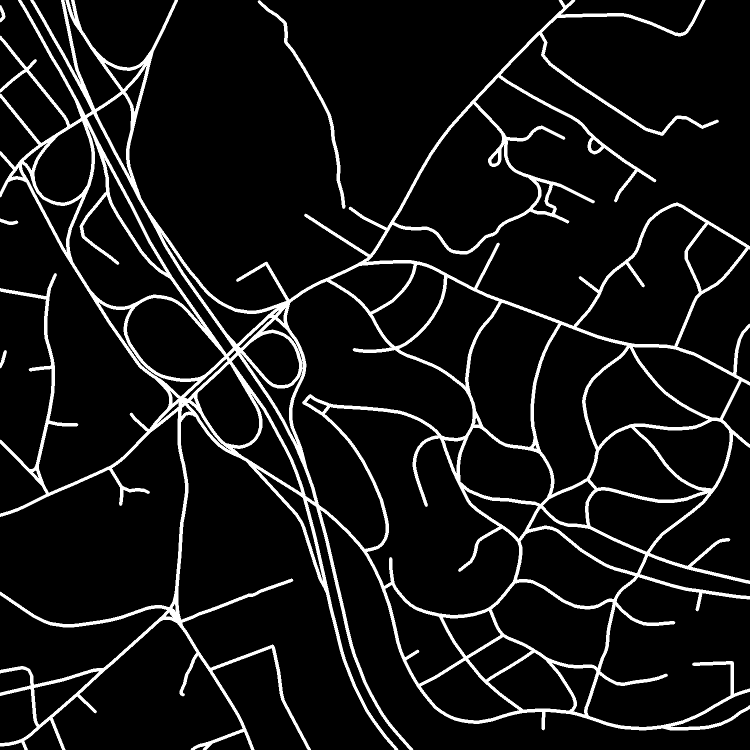
\includegraphics[width=\linewidth]{figs/datasets/Mass_roads_label_example2.png}
\caption{Label image} \label{fig:mass_roads_example_label}
\end{subfigure}
\hspace*{\fill} % separation between the subfigures
\caption{Example taken from test set in Massachusetts Roads Dataset} \label{fig:mass_roads_example}
\end{figure}


\todo[inline]{CRAPPY REWRITE. In regards to, dafuq!}
There are many reasons for using this dataset for conducting experiments related to the research questions.  The task involve semantic segmentation of roads based exclusively on aerial color images which is arguable a hard task, and might justify the use of a large model for training, such as a \ac{CNN}. Additionally, the labels have been generated from existing map data, and therefore contains many instances of naturally occurring inconsistent labelling. This is compelling in regards to the research questions of this thesis. The dataset has also been used in other works, which enables comparisons between the results obtained in this thesis and results obtained in other works. \\

\todo[inline]{Make into sentences}
Challenges \\
	Omission noise. Missing roads. Example\\
	Registration noise. Labels do not cover the roads in many instances.\\



%\subsection{Massachusetts Roads Dataset}
\todo[inline]{Include buildings dataset or not?}
\subsection{Norwegian Roads Dataset}
\todo[inline]{Fortid eller nåtid. You dummy?}
In addition to the Massachusetts Roads Dataset \citep{MnihThesis}, the proposed methods have been tested with the Norwegian Roads Dataset. This dataset was constructed from aerial images retrieved from Kartverket, which depicts both rural, suburban and urban areas from different locations in Norway. The entire dataset consists of 1225 aerial images, each being $1536\times 1536$ pixels in size. 1100 of the images have been randomly assigned to the training set, 75 the test set, and the remaining images were put in the validation set. Even though there are more aerial the images in this dataset compared to the Massachusetts Roads Dataset, it only covers an area of 1910 square kilometers. This is because of a much lower \ac{GSD} of about 0.66 meters per pixel. \\


The label images for this dataset have been generated from road centerline vectors found in the publicly available topographic vector database, N50, provided by \cite{Kartverket}. Unlike the Massachusetts Roads Dataset, the centerline vectors have been rasterized with a variable line thickness. This is possible because all road segment in N50 have different properties, which can be utilized when setting the line thickness. The actual thickness for each road types have been based on numbers found in a road specification manual published by The Norwegian Public Roads Administration \citep{Norwegian_road_manual}. The different type of roads, rules and line thickness for each road type are listed in Table \ref{tab:road_rules}. Roads which are underground and can not be seen from aerial imagery, have also been removed from the rasterized label images. \todo{Find property in table}\\

The aerial images have been taken from over 30 different locations in Norway, and offers a large variety of topographical features. There are images depicting coastline, rivers, mountain terrain, snow, cultivated land and forests. Compared to Massachusetts Roads Dataset the aerial images of this dataset have been sampled from a much larger areas. \\

Furthermore, the aerial images might present a challenge in terms of image quality. Some of the images have a lower quality, and differs in color balance, and contrast. There are also images which have been stitched together from  images captured by different flyovers \todo{CHECK what the heck this should be. OUTRAGEOUS}.\\  

The quality of the the generated label maps might also present a challenge to a machine learning algorithm. There are both omission and registration errors present in many of the label images. Compared to Massachusetts Roads Dataset there are a much higher degree of registration errors. The road centerlines in N50 generally appear more coarse, and result in less overlap between roads in the aerial image and the raster lines in the label image. This is especially evident in road centerline vectors for divided highways. Instead of having centerline vectors for both roadways, there are only one placed between the roadways on the median. Visual examples of missing and misplaced labels can be seen in Figure \ref{fig:norwegian_roads_examples_n50}.\\

\begin{figure}[h]
\begin{subfigure}{0.31\textwidth}
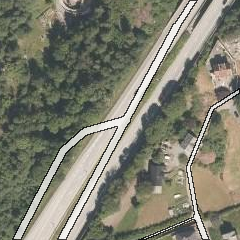
\includegraphics[width=\linewidth]{figs/datasets/nor_examples/1191_highway_n50.png}
\caption{Divided highways} \label{fig:norwegian_roads_highway_n50}
\end{subfigure}
\hspace*{\fill} % separation between the subfigures
\begin{subfigure}{0.31\textwidth}
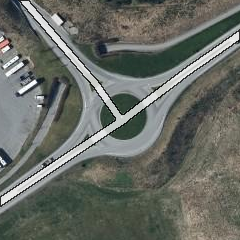
\includegraphics[width=\linewidth]{figs/datasets/nor_examples/1177_roundabout_n50.png}
\caption{Roundabout} \label{fig:norwegian_roads_roundabout_n50}
\end{subfigure}
\hspace*{\fill} % separation between the subfigures
\begin{subfigure}{0.31\textwidth}
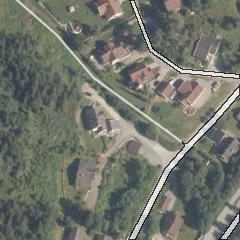
\includegraphics[width=\linewidth]{figs/datasets/nor_examples/1157_missing_n50.png}
\caption{Private road} \label{fig:norwegian_roads_missing_n50}
\end{subfigure}
\hspace*{\fill} % separation between the subfigures
\caption{Examples of label inconsistent labelling found in the Norwegian Roads Dataset N50} \label{fig:norwegian_roads_examples_n50}
\end{figure}

In addition to the set of label images generated from N50, the dataset also include an alternate set of label images generated from the topographic vector database, Vbase, which have more accurate road centerline vectors. There are still omission and registration errors present in this label image set, but to a less extent. Surfaces that share spectral similarities to asphalt, such as private roads and parking areas have not been marked, similar to the Massachusetts Roads Dataset. The difference in accuracy between N50 and Vbase, can be seen by comparing Figure \ref{fig:norwegian_roads_examples_n50} and Figure \ref{fig:norwegian_roads_examples_vbase}. A minor downside of using this vector database is that Vbase provide fewer road segment properties, which result in coarser raster line thicknesses \todo{My god, how dull!}.\\

\begin{figure}[h]
\begin{subfigure}{0.31\textwidth}
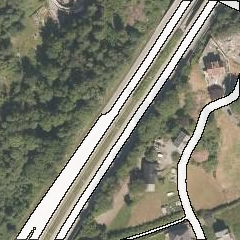
\includegraphics[width=\linewidth]{figs/datasets/nor_examples/1191_highway_vbase.png}
\caption{Divided highways} \label{fig:norwegian_roads_highway_vbase}
\end{subfigure}
\hspace*{\fill} % separation between the subfigures
\begin{subfigure}{0.31\textwidth}
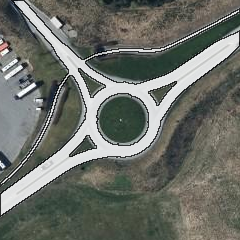
\includegraphics[width=\linewidth]{figs/datasets/nor_examples/1177_roundabout_vbase.png}
\caption{Roundabout} \label{fig:norwegian_roads_roundabout_vbase}
\end{subfigure}
\hspace*{\fill} % separation between the subfigures
\begin{subfigure}{0.31\textwidth}
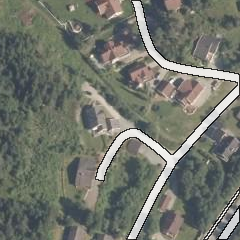
\includegraphics[width=\linewidth]{figs/datasets/nor_examples/1157_missing_vbase.png}
\caption{Private road} \label{fig:norwegian_roads_missing_vbase}
\end{subfigure}
\hspace*{\fill} % separation between the subfigures
\caption{Examples of road centerline vector quality in Vbase} \label{fig:norwegian_roads_examples_vbase}
\end{figure}

\begin{table}[htp]
\caption{Raster line thickness and road segment filtering rule for each type of road. The line thicknesses include a margin of 10\% compared to the numbers found in the road specification manual.}
\begin{center}
\begin{adjustbox}{max width=\textwidth}
\begin{tabular}{|c|l|r|}\hline
 		 Road type & Road segment property & line thickness\\\hline
 		 Dirt road & - & 2.50 m\\\hline
 		 Trail & - & 1.50 m\\\hline
 		 Private road & - & 3.50 m\\\hline
 		 pedestrian road & - & 2.25 m\\\hline
 		 Highway & MOTORVEGTYPE=motorveg & 10.80 m\\\hline
 		 International E-road network & VEGKATEGORI=E & 6.30 m\\\hline
 		 Norwegian national road & VEGKATEGORI=R & 5.85 m\\\hline
 		 municipal road & VEGKATEGORI=K & 4.95 m\\\hline
\end{tabular}
\end{adjustbox}
\end{center}
\label{tab:road_rules}
\end{table}

The dataset were constructed by using QGIS, an open source geographic information system application. The application enables viewing and editing of map data, but also provides a Python interface. A script to create label images was developed, which takes the map coordinates associated with each corner of an aerial image, and generates a raster image of road centerline vectors found inside that area. The resulting raster images can be used as target maps in supervised learning. \\

\begin{figure}
\begin{subfigure}{0.32\textwidth}
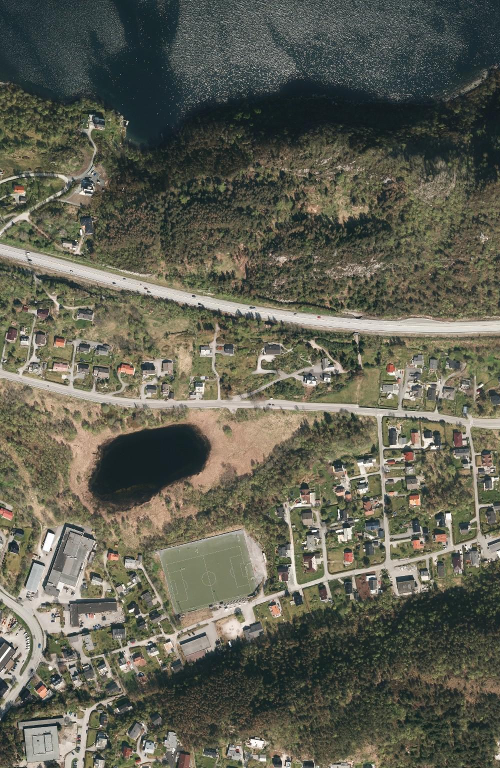
\includegraphics[width=\linewidth]{figs/datasets/Norwegian_roads_data_example2.png}
\caption{Aerial image} \label{fig:norwegian_roads_example_data}
\end{subfigure}
\hspace*{\fill} % separation between the subfigures
\begin{subfigure}{0.32\textwidth}
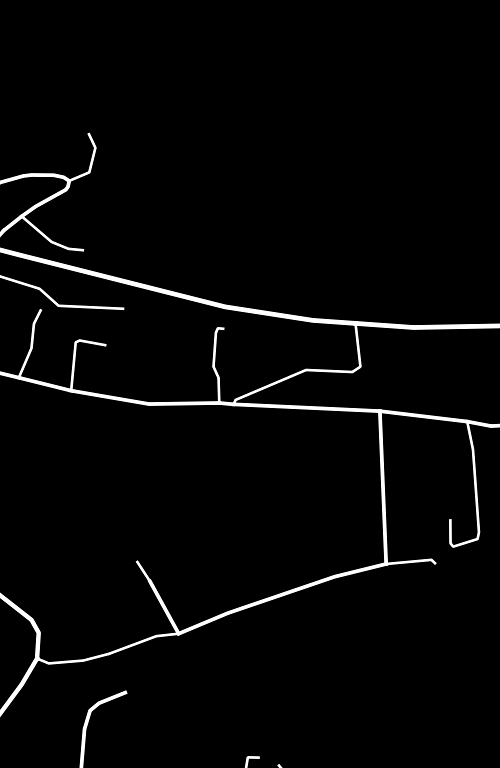
\includegraphics[width=\linewidth]{figs/datasets/Norwegian_roads_label_example2.png}
\caption{Label image} \label{fig:norwegian_roads_example_label}
\end{subfigure}
\hspace*{\fill} % separation between the subfigures
\begin{subfigure}{0.32\textwidth}
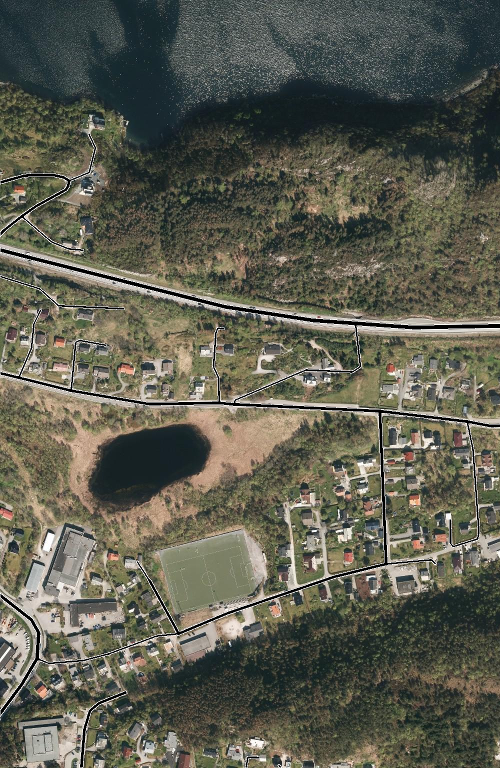
\includegraphics[width=\linewidth]{figs/datasets/Norwegian_roads_overlay_example2.png}
\caption{Overlay image} \label{fig:norwegian_roads_example_overlay}
\end{subfigure}
\hspace*{\fill} % separation between the subfigures
\caption{Example taken from test set in Norwegian Roads Dataset N50} \label{fig:norwegian_roads_example}
\end{figure}

An aerial image and it's corresponding label image from the Norwegian Roads Dataset can be seen in Figure \ref{fig:norwegian_roads_example}, and Figure \ref{fig:norwegian_roads_example_overlay} shows the same label image superimposed on the aerial image. Observe that some roads are missing from the label image, as well as the ground truth not covering the roads properly. \\
